The first step in our approach is to choose an existing SRL training corpus and align it to a large external database; for these we chose PropBank (PB) and Freebase~\cite{bollacker_freebase:_2008} (FB) respectively.
PropBank is an annotation layer on top of the Wall Street Journal portion of Penn Treebank II~\cite{marcus_building_1993}; for this reason, we expected better alignment if we only aligned PB to the business domain of FB.
We extracted the schema and predicate instances from PB using the Natural Language Toolkit~\cite{bird_nltk:_2006} and we retrieved the schema and relation instances from the business domain of FB from data dumps available on the FB web site.
Furthermore, we limited our alignment only to the most common predicates from PB.  The following figures illustrate the frequencies of common PB predicates and FB relations.

\begin{figure} [ht]

\begin{center}
{\label{avgstalls_CIF}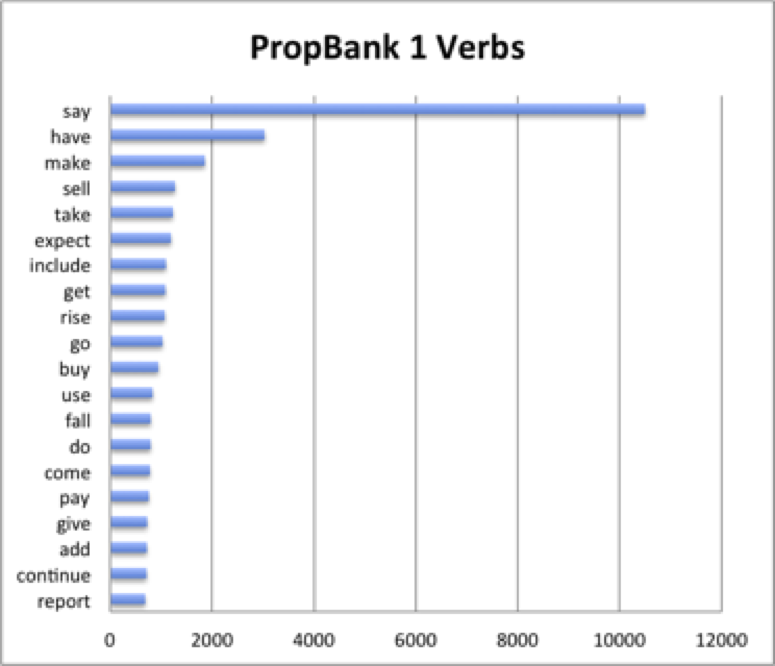
\includegraphics[width = 2in, height = 1.5in]{propverbs.png}}
\caption{Propbank Verbs}
\vspace{-0.5cm}
\label{}
\end{center}
\end{figure}

\begin{figure} [ht]
\begin{center}
{\label{avgstalls_CIF}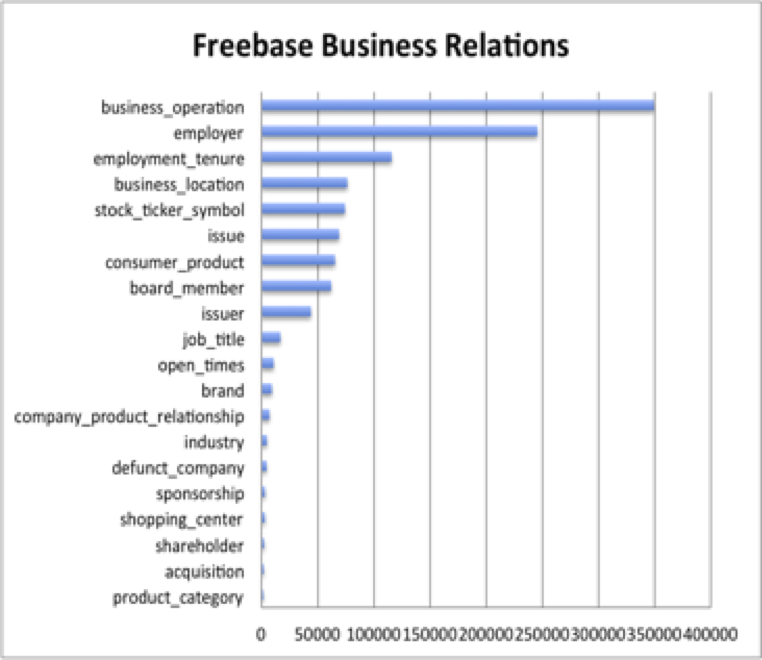
\includegraphics[width = 2in, height = 1.5in]{freebaserels.png}}
\caption{Freebase Relations}
\vspace{-0.5cm}
\label{}
\end{center}
\end{figure}

The following table shows predicates and relations we expected to be aligned.

\begin{table} [ht]
\begin{center}
\small{
\begin{tabular}{p{3cm}p{4cm}p{4.5cm}}
\noalign{\smallskip}
\hline
Area & Propbank Verbs & Freebase Relations\\	
\hline
Advising & advise & company\_ advisor \\
Employment & employ, hire & employment\_ tenure, employer\\
Products & make, produce, market, sell & company\_product\_relationship\\
Purchasing	& acquire, purchase, sell	& acquisition\\
Sponsors	&sponsor	&sponsorship\\
Stock	&issue&	issue\\
\hline
\end{tabular}
}
\caption{Aligning Propbank verbs to Freebase relations}
\vspace{-0.4cm}
\end{center}
\end{table}

Our goal for alignment was to generate automatically mappings between the PB and FB at the schema level for relations and the arguments of the relations; for example the PB predicate acquire may map to the FB relation acquisition.
Furthermore, acquire has a roleset acquire.01 - in general, PB predicates may have multiple rolesets - which defines four numbered arguments including the agent acquiring something, the thing acquired and the price paid.
And, the FB relation acquisition has the arguments acquiring\_company and company\_acquired.
In this example, we want to align agent from PB to acquiring\_company from FB, etc. 

We performed the alignment using a probabilistic soft logic (PSL) program~\cite{brocheler_probabilistic_2012} comprising the data loaded from PB and FB, and logical rules which act as templates for a constrained continuous Markov random field.
The variables in the graphical model for a PSL program are real-valued, making it ideal for propagating similarity, such as string similarities, at the instance level between the two data sources to the schema level, which was our goal; and inferences are assigned truth values which allow us to set a minimum threshold to accept mappings.
We encoded the following three types of alignment rules in PSL.
(i) Using Levenshtein similarity to capture similarity between relation names, entity names and entity type names.
(ii) Transitivity:  if relation A is similar to relation B, and relation B to relation C, relation A and C are similar.
And (iii) Set similarity:  if the sets of instances of two relations are similar, then the relations are similar.
We now share two specific PSL rules that we used, and explanations of how they work.
\begin{align}
w_{1}: rel(I1,R1)\wedge rel(I2,R2) \wedge similar(R1,R2)&\rightarrow sameRel(R1,R2) \label{eq:rel_name}\\
w_{1}: rel(I1,R1)\wedge rel(I2,R2) \wedge similar(\left\{R1.entOf(inv)\right\},\left\{R2.entOf(inv)\right\}) &\rightarrow sameRel(R1, R2) \label{eq:ent_set}
\end{align}
% I made these rules simpler here so they would render nicely in latex.  -- Alex
In rule~\eqref{eq:rel_name} two relations R1 and R2 from PB and FB respectively are same relations if they are similar. Similarity is calculated using Levenshtein distance.
Rule~\eqref{eq:ent_set} is the set similarity feature in PSL used to compare two sets of values.
Here we compare the arguments of propbank to arguments of freebase and indicate a match if arguments are similar.
Instead of comparing each and every argument, a single rule in PSL can be used for comparing the sets.
Both rules have weight $w_1 = 20$.

The following table shows example output of our alignment on relations; upon inspection, it appears that mappings with higher truth values are quite close to what we expect.
Notably, the mapping between hire and employment was inferred through the transitive rule and similarity in argument instances, though the predicate and relation have dissimilar names.

\begin{table} [ht]
\begin{center}
\small{
\begin{tabular}{p{3cm}p{3cm}p{2cm}}
\noalign{\smallskip}
\hline
PB Predicate & FB Relation & Truth Value\\	
\hline
issue & issue & 1.0 \\
issue &issuer & 0.99  \\
issue & holding & 0.97\\
employ	& employment	& 0.97\\
acquire	&acquisition	& 0.96\\
sponsor	&sponsorship&	 0.96\\
produce	&company\_product&	0.95\\
market	&employment &	0.94\\
issue	&employment &	0.94\\
sponsor & company\_advisor & 0.94\\
issue & company\_advisor & 0.94\\
advise & company\_advisor & 0.94\\
issue & asset\_ownership & 0.94\\
hire & employment & 0.87\\

\hline
\end{tabular}
}
\caption{PSL Alignment Predictions}
\vspace{-0.4cm}
\end{center}
\end{table}



